\documentclass[11pt]{article}
\usepackage[fontsize = 12pt]{scrextend}
\usepackage{multicol}
\usepackage{multirow}
\usepackage{savesym}
\usepackage{hyperref}
\usepackage{amsmath}
\usepackage{algorithm}
\usepackage{algorithmic}
\usepackage{paralist}
\usepackage{float}
\usepackage{bm}
\usepackage[shortlabels]{enumitem}
\usepackage[bb=px]{mathalpha}
\usepackage[a4paper, margin=1in]{geometry}
\usepackage[dvipsnames]{xcolor}
\usepackage{tikz}
\newtheorem{theorem}{Theorem}
\usetikzlibrary{shapes,backgrounds}
\usetikzlibrary{positioning}
\title{SDS 383C - Statistical Modeling 1: Homework 3}
\author{Rahul Nandakumar \\ Graduate Student, ORIE Program (E-ID: rn9355)}
\date{October 20, 2022}
\begin{document}
\maketitle
\noindent \emph{1.}\\ \\
\textbf{Solution:} It is given that $\mathbf{y_{1}, \dots y_{n}} \overset{iid}{\sim} p(\mathbf{y \text{ }|\text{ } \bm{\theta}}) = h(\mathbf{y})\text{exp}\{\bm{\theta}^{T}\mathbf{y} - \psi(\bm{\theta})\}$\\ \\
\emph{a.} We need to prove that
\begin{equation}
  \nonumber
  \mathbb{E}(\mathbf{y} \text{ }|\text{ } \bm{\theta}) = \bm{\xi}({\bm{\theta}}) = \frac{\partial \psi(\bm{\theta})}{\partial \bm{\theta}}
\end{equation}
Using the property of probability distributions, that is the area under the pdf over the support = 1
\begin{equation}
  \nonumber
  \begin{aligned}
    \int_{-\infty}^{\infty} p(\mathbf{y \text{ }|\text{ } \bm{\theta}})d\mathbf{y} & = 1\\
    \Rightarrow \frac{d}{d \bm{\theta}} \int_{-\infty}^{\infty} p(\mathbf{y \text{ }|\text{ } \bm{\theta}})d\mathbf{y} & = 0; \text{ Taking derivative w.r.t }\bm{\theta}\text{ on both sides}
  \end{aligned}
\end{equation}
Using Leibniz Integral rule, which is given as follows,
\begin{equation}
  \nonumber
  \begin{aligned}
    \frac{d}{dx} \int_{a(x)}^{b(x)} f(x, t)dt & = f(x, b(x))\frac{d}{dx}b(x) - f(x, a(x))\frac{d}{dx}a(x) + \int_{a(x)}^{b(x)}\frac{\partial}{\partial x}f(x,t)dt
  \end{aligned}
\end{equation}
When $a(x) = a$ and $b(x) = b$, we get
\begin{equation}
  \nonumber
  \begin{aligned}
    \frac{d}{dx} \int_{a}^{b} f(x, t)dt & = \int_{a}^{b}\frac{\partial}{\partial x}f(x,t)dt
  \end{aligned}
\end{equation}
Using this result in our equation, we get
\begin{equation}
  \nonumber
  \begin{aligned}
    \Rightarrow & \frac{d}{d \bm{\theta}} \int_{-\infty}^{\infty} p(\mathbf{y \text{ }|\text{ } \bm{\theta}})d\mathbf{y} = 0\\
    \Rightarrow & \int_{-\infty}^{\infty} \frac{\partial}{\partial \bm{\theta}}p(\mathbf{y \text{ }|\text{ } \bm{\theta}})d\mathbf{y} = 0\\
    \Rightarrow & \int_{-\infty}^{\infty} \frac{\partial}{\partial \bm{\theta}}h(\mathbf{y})\text{e}^{\bm{\theta}^{T}\mathbf{y} - \psi(\bm{\theta})}d\mathbf{y} = 0\\
    \Rightarrow & \int_{-\infty}^{\infty} h(\mathbf{y})\text{e}^{\bm{\theta}^{T}\mathbf{y} - \psi(\bm{\theta})}\bigg(\mathbf{y} - \frac{\partial}{\partial \bm{\theta}}\psi(\bm{\theta})\bigg)d\mathbf{y} = 0\\
  \end{aligned}
\end{equation}
\begin{equation}
  \nonumber
  \begin{aligned}
    \Rightarrow & \int_{-\infty}^{\infty} \mathbf{y}h(\mathbf{y})\text{e}^{\bm{\theta}^{T}\mathbf{y} - \psi(\bm{\theta})}d\mathbf{y} - \int_{-\infty}^{\infty} h(\mathbf{y})\text{e}^{\bm{\theta}^{T}\mathbf{y} - \psi(\bm{\theta})} \bigg(\frac{\partial}{\partial \bm{\theta}}\psi(\bm{\theta})\bigg)d\mathbf{y} = 0\\
    \Rightarrow & \mathbb{E}(\mathbf{y} | \bm{\theta}) - \frac{\partial}{\partial \bm{\theta}}\psi(\bm{\theta})\int_{-\infty}^{\infty} h(\mathbf{y})\text{e}^{\bm{\theta}^{T}\mathbf{y} - \psi(\bm{\theta})}d\mathbf{y} = 0\\
    \Rightarrow & \mathbb{E}(\mathbf{y} | \bm{\theta}) = \frac{\partial}{\partial \bm{\theta}}\psi(\bm{\theta}); \text{ Since }\int_{-\infty}^{\infty} h(\mathbf{y})\text{e}^{\bm{\theta}^{T}\mathbf{y} - \psi(\bm{\theta})}d\mathbf{y} = 1. \text{ \emph{\underline{Hence proved (a.)}}}
  \end{aligned}
\end{equation}
\emph{b.} Now we have,
\begin{equation}
  \nonumber
  p(\bm{\theta} \text{ }| \text{ } \mathbf{y}_{0}, \lambda) = h(\mathbf{y}_{0}, \lambda)\text{exp}\{\bm{\theta}^{T}\mathbf{y}_{0} - \lambda \psi(\bm{\theta})\}
\end{equation}
We know that,
\begin{equation}
  \nonumber
  \begin{aligned}
    & \int_{-\infty}^{\infty} p(\bm{\theta} \text{ }| \text{ } \mathbf{y}_{0}, \lambda)d\bm{\theta} = 1\\
    \Rightarrow & \frac{d}{d \bm{\theta}} \int_{-\infty}^{\infty} p(\bm{\theta} \text{ }| \text{ } \mathbf{y}_{0}, \lambda)d\bm{\theta} = 0; \text{ Taking derivative on both sides wrt } \bm{\theta}\\
    \Rightarrow & \frac{d}{d \bm{\theta}} \int_{-\infty}^{\infty} h(\mathbf{y}_{0}, \lambda)e^{\bm{\theta}^{T}\mathbf{y}_{0} - \lambda \psi(\bm{\theta})}d\bm{\theta} = 0\\
    \Rightarrow &  \int_{-\infty}^{\infty} \frac{\partial}{\partial \bm{\theta}} h(\mathbf{y}_{0}, \lambda)e^{\bm{\theta}^{T}\mathbf{y}_{0} - \lambda \psi(\bm{\theta})}d\bm{\theta} = 0; \text{ Applying Leibniz rule as stated above}\\
    \Rightarrow &  \int_{-\infty}^{\infty} h(\mathbf{y}_{0}, \lambda)e^{\bm{\theta}^{T}\mathbf{y}_{0} - \lambda \psi(\bm{\theta})}\bigg(\mathbf{y}_{0} - \lambda \frac{\partial}{\partial \bm{\theta}} \psi(\bm{\theta}) \bigg)d\bm{\theta} = 0\\
    \Rightarrow &  \int_{-\infty}^{\infty} \mathbf{y}_{0}h(\mathbf{y}_{0}, \lambda)e^{\bm{\theta}^{T}\mathbf{y}_{0} - \lambda \psi(\bm{\theta})}d\bm{\theta} - \int_{-\infty}^{\infty}h(\mathbf{y}_{0}, \lambda)e^{\bm{\theta}^{T}\mathbf{y}_{0} - \lambda \psi(\bm{\theta})}\bigg(\lambda \frac{\partial}{\partial \bm{\theta}} \psi(\bm{\theta}) \bigg)d\bm{\theta} = 0\\
  \end{aligned}
\end{equation}
Since we know that
\begin{equation}
  \nonumber
  \int_{-\infty}^{\infty} h(\mathbf{y}_{0}, \lambda)e^{\bm{\theta}^{T}\mathbf{y}_{0} - \lambda \psi(\bm{\theta})}d\bm{\theta} = 1
\end{equation}
and
\begin{equation}
  \nonumber
  \int_{-\infty}^{\infty}h(\mathbf{y}_{0}, \lambda)e^{\bm{\theta}^{T}\mathbf{y}_{0} - \lambda \psi(\bm{\theta})}\bigg(\frac{\partial}{\partial \bm{\theta}} \psi(\bm{\theta}) \bigg)d\bm{\theta} = \mathbb{E}\bigg(\frac{\partial}{\partial \bm{\theta}}\psi(\bm{\theta})\bigg)
\end{equation}
\begin{equation}
  \nonumber
  \begin{aligned}
    \Rightarrow & \mathbf{y}_{0}(1) = \lambda\mathbb{E}\bigg(\frac{\partial}{\partial \bm{\theta}}\psi(\bm{\theta})\bigg) + c\\
    \Rightarrow & \mathbb{E}\bigg(\frac{\partial}{\partial \bm{\theta}}\psi(\bm{\theta})\bigg) = \frac{\mathbf{y}_{0}}{\lambda} + c\\
    \Rightarrow & \mathbb{E}(\bm{\xi}({\bm{\theta}})) = \frac{\mathbf{y}_{0}}{\lambda} + c. \text{ \emph{\underline{Hence proved (b.)}}}
  \end{aligned}
\end{equation}
Another way to think of this result is to use the hint given that,
\begin{equation}
  \nonumber
  \frac{\partial \psi(\bm{\theta})}{\partial \bm{\theta}} = \frac{1}{\lambda}\bigg\{\mathbf{y}_{0} - \bigg(\mathbf{y}_{0} - \lambda\frac{\partial \psi(\bm{\theta})}{\partial \bm{\theta}} \bigg)\bigg\}
\end{equation}
Let us consider the expectation of this expression on both sides (w.r.t $p(\bm{\theta} \text{ }|\text{ } \mathbf{y}_{0}, \lambda)$).
\begin{equation}
  \nonumber
  \begin{aligned}
    \mathbb{E}\bigg(\frac{\partial \psi(\bm{\theta})}{\partial \bm{\theta}}\bigg) & = \mathbb{E}\bigg(\frac{\mathbf{y}_{0}}{\lambda}\bigg) - \frac{1}{\lambda}\mathbb{E}\bigg(\mathbf{y}_{0} - \lambda \frac{\partial \psi(\bm{\theta})}{\partial \bm{\theta}} \bigg)\\
    & = \bigg(\frac{\mathbf{y}_{0}}{\lambda}\bigg) - \frac{1}{\lambda} \int_{-\infty}^{\infty} \bigg(\mathbf{y}_{0} - \lambda \frac{\partial \psi(\bm{\theta})}{\partial \bm{\theta}} \bigg)\times p(\bm{\theta} \text{ }|\text{ } \mathbf{y}_{0}, \lambda) d \bm{\theta}\\
    & = \bigg(\frac{\mathbf{y}_{0}}{\lambda}\bigg) - \frac{1}{\lambda} \int_{-\infty}^{\infty} \bigg(\mathbf{y}_{0} - \lambda \frac{\partial \psi(\bm{\theta})}{\partial \bm{\theta}} \bigg)\times h(\mathbf{y}_{0}, \lambda)\text{exp}\{\bm{\theta}^{T}\mathbf{y}_{0} - \lambda \psi(\bm{\theta})\} d \bm{\theta}\\
    & = \bigg(\frac{\mathbf{y}_{0}}{\lambda}\bigg) - \frac{h(\mathbf{y}_{0}, \lambda)}{\lambda} \times c
  \end{aligned}
\end{equation}
Note that this can be done because if we assume $\bm{\theta}^{T}\mathbf{y}_{0} - \lambda \psi(\bm{\theta}) = k$, then $(\mathbf{y}_{0} - \lambda \frac{\partial \psi(\bm{\theta})}{\partial \bm{\theta}}) d \bm{\theta} = dk$. Now, $\int_{-\infty}^{\infty} \text{exp}\{k\} dk$ equates to a constant as k  may occupy any value in the support. Therefore, our final expression becomes,
\begin{equation}
  \nonumber
  \begin{aligned}
    \mathbb{E}(\bm{\xi}({\bm{\theta}})) = \frac{\mathbf{y}_{0}}{\lambda} + c.
  \end{aligned}
\end{equation}
\emph{c.} Now, we need to show that
\begin{equation}
  \nonumber
  \mathbb{E}(\bm{\xi}(\bm{\theta}) \text{ }|\text{ } y_{1:n}) = \frac{\mathbf{y_{0}} + n\bar{\mathbf{y}}}{\lambda + n} + \text{constant}
\end{equation}
We have,
\begin{equation}
  \nonumber
  \begin{aligned}
    p(\bm{\theta} \text{ }|\text{ } y_{1:n}) & \propto p(\bm{\theta}) \times p(y_{1:n} \text{ }|\text{ } \bm{\theta})\\
    & \propto p(\bm{\theta} \text{ }| \text{ } \mathbf{y}_{0}, \lambda) \times p(y_{1:n} \text{ }|\text{ } \bm{\theta})\\
    & \propto h(\mathbf{y}_{0}, \lambda)e^{\bm{\theta}^{T}\mathbf{y}_{0} - \lambda \psi(\bm{\theta})} \times \prod_{i = 1}^{n} h(\mathbf{y}_{i})e^{\bm{\theta}^{T}\mathbf{y}_{i} - \psi(\bm{\theta})}\\
    & \propto h(\mathbf{y}_{0}, \lambda) \times \prod_{i = 1}^{n} h(\mathbf{y}_{i})\times e^{\bm{\theta}^{T}(\mathbf{y}_{0} + \sum_{i = 1}^{n}y_{i}) - \psi(\bm{\theta})(\lambda + \sum_{i = 1}^{n}1)}\\
    & \propto h'(\mathbf{y}_{0}, \lambda) e^{\bm{\theta}^{T}(\mathbf{y}_{0} + n\bar{\mathbf{y}}) - \psi(\bm{\theta})(\lambda + n)}\\
  \end{aligned}
\end{equation}
We observe that this pdf is similar to the previous question, where $p(\bm{\theta} \text{ }| \text{ } \mathbf{y}_{0}, \lambda) = h(\mathbf{y}_{0}, \lambda)\text{exp}\{\bm{\theta}^{T}\mathbf{y}_{0} - \lambda \psi(\bm{\theta})\}$. Here, we proved that
\begin{equation}
  \nonumber
  \mathbb{E}(\bm{\xi}({\bm{\theta}})) = \frac{\mathbf{y}_{0}}{\lambda} + c
\end{equation}
By appealing to a similar conjugacy and by comparing the distributions, we can say that for this distribution $p(\bm{\theta} \text{ }|\text{ } y_{1:n})$
\begin{equation}
  \nonumber
  \mathbb{E}(\bm{\xi}(\bm{\theta}) \text{ }|\text{ } y_{1:n}) = \frac{\mathbf{y_{0}} + n\bar{\mathbf{y}}}{\lambda + n} + \text{constant}
\end{equation}
\\ \\
\emph{2}. Show that the binomial and negative binomial distributions belong to exponential families.\\ \\
\textbf{Solution: }The exponential family of distributions is characterized by having the probability distribution in the form,
\begin{equation}
  \nonumber
  p(\mathbf{y} \text{ }|\text{ }\bm{\theta}) = h(\mathbf{y})\text{exp}\{\phi(\bm{\theta})^{T}\mathbf{u(y)} - \psi(\bm{\theta})\}
\end{equation}
Let us consider a binomial distribution,
\begin{equation}
  \nonumber
  y_{1} \dots y_{n} \overset{iid}{\sim} Bin(n, \theta)
\end{equation}
Let the probability of success is $\theta$. The pmf of this distribution is given by,
\begin{equation}
  \nonumber
  \begin{aligned}
    p(y | \theta) & = {n \choose y}(\theta)^{y}(1 - \theta)^{n-y}\\
    & = {n \choose y} e^{log\big((\theta)^{y}(1 - \theta)^{n-y}\big)}\\
    & = {n \choose y} e^{(y)log(\theta) + (n-y)log(1-\theta)}\\
    & = {n \choose y} e^{(y)(log(\theta) - log(1 - \theta)) + (n)log(1-\theta)}\\
    & = {n \choose y} e^{(y)(log\frac{\theta}{1 - \theta}) + (n)log(1-\theta)}\\
  \end{aligned}
\end{equation}
Here, the following similarities are observed with the exponential family of distributions.
\begin{equation}
  \nonumber
  \begin{aligned}
    \phi(\bm{\theta})^{T} & = log\frac{\theta}{1 - \theta}\\
    \mathbf{u(y)} & = y\\
    h(\mathbf{y}) & = {n \choose y}\\
    \psi(\bm{\theta}) & = -nlog(1 - \theta)
  \end{aligned}
\end{equation}
Therefore, we can conclude that the binomial distributions belongs to exponential family of distributions. Now, let us consider the negative binomial distribution. Described as the probability of getting $k$ failures before $r$ successes, this pmf is given by,
\begin{equation}
  \nonumber
  \begin{aligned}
    p(k | r,\theta) & = {k + r - 1 \choose r-1}(\theta)^{r}(1 - \theta)^{k}\\
    & = {k + r - 1 \choose r-1}e^{log\big((\theta)^{r}(1 - \theta)^{k}\big)}\\
    & = {k + r - 1 \choose r-1}e^{(k)log(1-\theta) + (r)log(\theta)}
  \end{aligned}
\end{equation}
Here, the following similarities are observed with the exponential family of distributions.
\begin{equation}
  \nonumber
  \begin{aligned}
    \phi(\bm{\theta})^{T} & = log(1 - \theta)\\
    \mathbf{u(y)} & = k\\
    h(\mathbf{y}) & = {k + r - 1 \choose r - 1}\\
    \psi(\bm{\theta}) & = -(r)log(\theta)
  \end{aligned}
\end{equation}
Therefore, we can conclude that the negative binomial distributions belongs to exponential family of distributions.\\ \\
\emph{3.}\\ \\
\textbf{Solution:} \\ \\
\emph{a.} It is given that $y \sim Bin(10, \theta)$. We know that the likelihood function for the binomial distribution is given by
\begin{equation}
  \nonumber
  p(y_{1:n} \text{ }|\text{ } \theta) \propto \prod_{i = 1}^{n} \theta^{y_{i}}(1 - \theta)^{n-y_{i}}
\end{equation}
Here n = 10, and it is given that y = 3. Therefore, our likelihood function becomes,
\begin{equation}
  \nonumber
  p(y \text{ }|\text{ } \theta)  \propto \theta^{3}(1 - \theta)^{7}
\end{equation}
It is given that the prior is given by a mixture of two beta's as,
\begin{equation}
  \nonumber
  p(\theta) = \frac{0.5}{\text{Beta}(10,20)}\theta^{10-1}(1-\theta)^{20-1} + \frac{0.5}{\text{Beta}(20,10)}\theta^{20-1}(1-\theta)^{10-1}
\end{equation}
We know that,
\begin{equation}
  \nonumber
  \begin{aligned}
    p(\theta \text{ }|\text{ } y) & \propto p(y \text{ }|\text{ } \theta) \times p(\theta)\\
    & \propto [\theta^{3}(1 - \theta)^{7}] \times \bigg[\frac{0.5}{\text{Beta}(10,20)}\theta^{9}(1-\theta)^{19} + \frac{0.5}{\text{Beta}(20,10)}\theta^{19}(1-\theta)^{9}\bigg]\\
    & \propto \frac{0.5}{\text{Beta}(10,20)}\theta^{12}(1-\theta)^{26} + \frac{0.5}{\text{Beta}(20,10)}\theta^{22}(1-\theta)^{16}\\
    & = c \times \bigg[\frac{0.5}{\text{Beta}(10,20)}\theta^{12}(1-\theta)^{26} + \frac{0.5}{\text{Beta}(20,10)}\theta^{22}(1-\theta)^{16}\bigg]
  \end{aligned}
\end{equation}
Let c be a constant. We know that the posterior is proportional to the above expression, however, we are asked to find an exact value for the pdf. For this, we can utilize the idea that the total area under the density = 1, i.e.,
\begin{equation}
  \nonumber
  \begin{aligned}
    \int_{0}^{1} c \times \bigg[\frac{0.5}{\text{Beta}(10,20)}\theta^{12}(1-\theta)^{26} + \frac{0.5}{\text{Beta}(20,10)}\theta^{22}(1-\theta)^{16}\bigg] d\theta & = 1\\
    \frac{1}{\int_{0}^{1} \bigg[\frac{1}{\text{Beta}(10,20)}\theta^{12}(1-\theta)^{26} + \frac{1}{\text{Beta}(20,10)}\theta^{22}(1-\theta)^{16}\bigg] d\theta} & = c'; c' = c \times 0.5\\
  \end{aligned}
\end{equation}
Therefore, we get the value of c' as
\begin{equation}
  \nonumber
   c' = 2.1278644 \times 10^{-3}; \text{ I used Wolfram alpha calculator to obtain the integral value}
\end{equation}
Now, we can verify that
\begin{equation}
  \nonumber
  \frac{\text{Beta}(13,27)}{\text{Beta}(20,10)} + \frac{\text{Beta}(23,17)}{\text{Beta}(10,20)} = c' = 2.1278644 \times 10^{-3}
\end{equation}
Therefore, we can rewrite our posterior as,
\begin{equation}
  \nonumber
  p(\theta \text{ }|\text{ } y) = \frac{\frac{\text{Beta}(13,27)}{\text{Beta}(13,27)\text{Beta}(10,20)}\theta^{12}(1-\theta)^{26} + \frac{\text{Beta}(23,17)}{\text{Beta}(23,17)\text{Beta}(20,10)}\theta^{22}(1-\theta)^{16}}{\frac{\text{Beta}(13,27)}{\text{Beta}(20,10)} + \frac{\text{Beta}(23,17)}{\text{Beta}(10,20)}}; \text{\emph{ \underline{Hence Proved}}}
\end{equation}
\emph{b.} We plot the posterior superimposed on the prior as follows. The code accompanying this plot is explained and attached with this assignment.
\begin{figure}[H]
  \centering
  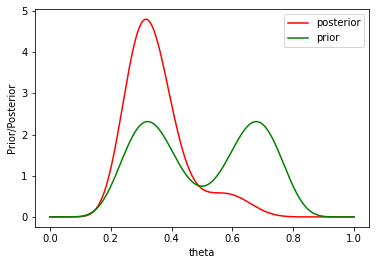
\includegraphics[width = 0.6\textwidth]{q3b.png}
  \caption{Posterior superimposed on the beta mixture prior}
\end{figure}
\noindent \emph{c.} We are asked to find a 90\% posterior credible intreval for $\theta$. Here, $\alpha = 0.1$. We do this in Python, using the Quantile based credible intrevals, as it was mentioned in the lecture notes that Quantile based credible intrevals are used much more in practice. It is defined as,
\begin{equation}
  \nonumber
  \begin{aligned}
    C_{\theta, \alpha} & = \{\theta : Pr(C_{\theta, \alpha \text{ }|\text{ } y_{1:n}}) = 1 - \alpha\}\\
    & = \{\theta_{n, 1 - \alpha_{1}} \leq \theta \leq \theta_{n, \alpha_{2}}, \alpha_{1} + \alpha_{2} = \alpha\}
  \end{aligned}
\end{equation}
We implement a function that calculates the inverse pdf values for our posterior distribution. Now using these values, we consider the 5th quantile and the 95th quantile values for the posterior distribution as this is essentially meaning that the probability of occurence of values in this intreval $\geq 90\%$. In these calculations, we generate 100000 values of $\theta$ and find the posterior distribution using the expression as above. By inputting these posterior distribution values, and by calculating the inverse pdf, we can get the values of $\theta$. From this, we can calculate the 5th and 95th quantiles, as here $\alpha_{1} = 0.05$. Our calculations leads us to a value of the quantiles as $q_{1} = 0.21266799901229458, q_{2} = 0.5844785401328614$. The graphical representation of this is also given below.
\begin{figure}[H]
  \centering
  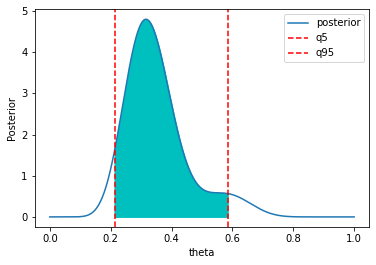
\includegraphics[width = 0.6\textwidth]{q3c.png}
  \caption{Quantile based credible regions}
\end{figure}
\noindent \emph{4.}\\ \\
\textbf{Solution:}
We are given that the Jeffry's prior is given by
\begin{equation}
  \nonumber
  p(\bm{\theta}) \propto |\mathbf{I}(\bm{\theta})|^{-\frac{1}{2}}
\end{equation}
Now, we consider a one-one function $\bm{\psi} = g(\bm{\theta})$. This implies, $\bm{\theta} = g^{-1}(\bm{\psi})$. Now, let us evaluate $\mathbf{I}(\bm{\psi})$ at this new $\bm{\theta} = g^{-1}(\bm{\psi})$. This gives us,
\begin{equation}
  \nonumber
  \begin{aligned}
    \mathbf{I}(\bm{\psi}) & = -\mathbb{E}\bigg(\frac{\partial^{2} \text{log } p(y | \bm{\psi})}{\partial {\bm{\psi}}^{2}}\bigg)\\
    & = -\mathbb{E}\bigg(\frac{\partial^{2} \text{log } p(y | \bm{\theta} = g^{-1}(\bm{\psi}))}{\partial {\bm{\theta}}^{2}}\bigg|\frac{d \bm{\theta}}{d \bm{\psi}}\bigg|^{2}\bigg)\\
    & = \mathbf{I}(\bm{\theta}) \bigg|\frac{d \bm{\theta}}{d \bm{\psi}}\bigg|^{2}
  \end{aligned}
\end{equation}
Computing the Jeffry's prior on $\bm{\psi} = g(\bm{\theta})$ from here, we get,
\begin{equation}
  \nonumber
  \begin{aligned}
    p(\bm{\psi}) & \propto |\mathbf{I}(\bm{\psi})|^{-\frac{1}{2}}\\
    & \propto \mathbf{I}(\bm{\theta}) \bigg|\frac{d \bm{\theta}}{d \bm{\psi}}\bigg|^{2}\\
    & \propto \mathbf{I}(\bm{\theta})
  \end{aligned}
\end{equation}
Thus, we are able to show that Jeffrey's priors satisfies the invariance principle.\\ \\
\emph{5.}\\ \\
\textbf{Solution:} It is given that
\begin{equation}
  \nonumber
  y_{1} \dots y_{n} \sim \text{Pois}(\lambda)
\end{equation}
The likelihood function is given by
\begin{equation}
  \nonumber
  p(y_{1:n} \text{ }|\text{ } \lambda) = \prod_{i = 1}^{n} \frac{e^{-\lambda}\lambda^{y_{i}}}{y_{i}!}
\end{equation}
We arrived at the Jeffry's prior for the Poisson distribution as,
\begin{equation}
  \nonumber
  p(\lambda) \propto \lambda^{\frac{-1}{2}}
\end{equation}
Now, we can calculate the posterior as follows,
\begin{equation}
  \nonumber
  \begin{aligned}
    p(\lambda \text{ }|\text{ } y_{1:n}) & \propto p(\lambda) \times p(y_{1:n} \text{ }|\text{ } \lambda)\\
    &  \propto  \prod_{i = 1}^{n} \frac{e^{-\lambda}\lambda^{y_{i}}}{y_{i}!} \times \lambda^{\frac{-1}{2}}\\
    & \propto (e^{-\lambda})^{n} \times \lambda^{y_{1}} \dots \lambda^{y_{n}} \times \lambda^{\frac{-1}{2}}\\
    & \propto e^{-n \lambda} \lambda^{y_{1} + \dots + y_{n} - \frac{1}{2}}
  \end{aligned}
\end{equation}
This posterior looks like the pmf of a Gamma distribution. We need to note that the distribution of the posterior is now in terms of $\lambda$. The Gamma distribution is given by,
\begin{equation}
  \nonumber
  f(x | \alpha, \beta) = \text{Gamma}(\alpha, \beta) = \frac{x^{\alpha - 1}e^{-\beta x} \beta^{\alpha}}{\Gamma(\alpha)}
\end{equation}
Essentially here, we can see that,
\begin{equation}
  \nonumber
  \begin{aligned}
    x & = \lambda\\
    \beta & = n\\
    \alpha & = y_{1} + \dots y_{n} + \frac{1}{2}
  \end{aligned}
\end{equation}
Therefore, we can conclude that the posterior is of the form Gamma($\alpha, \beta$), with $\alpha$ and $\beta$ as described above, and is a proper density.\\ \\
\emph{6.}\\ \\
\textbf{Solution:} It is given that,
\begin{equation}
  \nonumber
  y_{1},\dots,y_{n} \sim N(\mu, \sigma^{2})
\end{equation}
with $\mu$ being known.\\ \\
\emph{a.} The Jeffrey's prior for $\sigma^{2}$ can be calculated as follows. First, we calculate the likelihood function for $\sigma^{2}$. This has been done in previous homeworks, and we get
\begin{equation}
  \nonumber
  L(\sigma^{2}) = \prod_{i = 1}^{n} \frac{1}{\sqrt{2\pi}\sigma}e^{\frac{-1}{2\sigma^{2}} (y_{i} - \mu)^{2}}\\
\end{equation}
From this, we can arrive at the Fisher information matrix as,
\begin{equation}
  \nonumber
  \begin{aligned}
    \mathbf{I}(\sigma^{2}) & = -\mathbb{E}\bigg[\frac{\partial^{2} \mathcal{L}(\sigma^2)}{\partial (\sigma^{2})^{2}}\bigg]\\
    & = -\mathbb{E}\bigg[\frac{n}{2 \sigma^{4}} - \frac{1}{\sigma^{6}} \sum_{i = 1}^{n}(y_{i} - \mu)^{2}\bigg]\\
    & = -\bigg[\frac{n}{2 \sigma^{4}} - \frac{1}{\sigma^{6}} n\sigma^{2}\bigg]\\
    & = \frac{n}{2\sigma^{4}}
  \end{aligned}
\end{equation}
Therefore, the Jeffrey's prior for $\sigma^{2}$ is given as,
\begin{equation}
  \nonumber
  \begin{aligned}
    p(\sigma^{2}) & \propto |\mathbf{I}(\sigma^{2})|^{\frac{1}{2}}\\
    & \propto \bigg|\frac{n}{2\sigma^{4}}\bigg|\\
    & \propto \frac{1}{\sigma^{2}}
  \end{aligned}
\end{equation}
\emph{b.} We can compute the corresponding posterior using the following relation.
\begin{equation}
  \nonumber
  \begin{aligned}
    p(\sigma^{2} | y_{1:n}) & \propto p(y_{1:n} | \sigma^{2}) \times p(\sigma^{2})\\
    & \propto \prod_{i = 1}^{n} \frac{1}{\sqrt{2\pi}\sigma}e^{\frac{-1}{2\sigma^{2}} (y_{i} - \mu)^{2}} \times \frac{1}{\sigma^{2}}\\
    & \propto \prod_{i = 1}^{n} \frac{1}{\sqrt{2\pi}\sigma^{1 + \frac{2}{n}}}e^{\frac{-1}{2\sigma^{2}} (y_{i} - \mu)^{2}}\\
    & \propto \bigg(\frac{1}{\sqrt{2\pi}\sigma^{1 + \frac{2}{n}}}\bigg)^{n} \prod_{i = 1}^{n}e^{\frac{-1}{2\sigma^{2}} (y_{i} - \mu)^{2}}\\
    & \propto (\sigma^{2})^{-\frac{n}{2} - 1}e^{\frac{-1}{2\sigma^{2}} \sum_{i = 1}^{n} (y_{i} - \mu)^{2}}\\
  \end{aligned}
\end{equation}
This looks like the pdf of an inverse gamma distribution. The pdf of the inverse gamma distribution is given by
\begin{equation}
  \nonumber
  f(x | \alpha, \beta) = \frac{\beta^{\alpha}}{\Gamma(\alpha)}\bigg(\frac{1}{x}\bigg)^{\alpha+1}\text{exp}\bigg(\frac{-\beta}{x}\bigg)
\end{equation}
Our posterior is constructed with the following parameters,
\begin{equation}
  \nonumber
  \begin{aligned}
    \alpha & = \frac{n}{2}\\
    \beta & = \frac{\sum_{i = 1}^{n} (y_{i} - \mu)^{2}}{2}
  \end{aligned}
\end{equation}
\emph{c.}
First, we consider a Normal(0,1) distribution and then we draw a sample size of 20 from this distribution. Using this, we can calculate the value of $\alpha$ and $\beta$ for the posterior. We then plot the distribution of the posterior over the support $\sigma^{2}$ and superimpose it over the prior. The general shape of the prior is given by the following plot, for values of $\sigma^{2}$ between 0 and 1.
\begin{figure}[H]
  \centering
  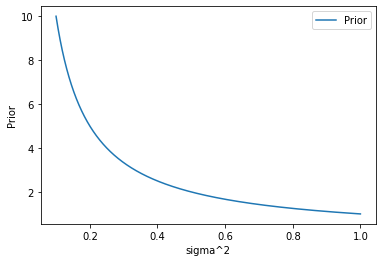
\includegraphics[width = 0.6\textwidth]{q6a.png}
  \caption{Prior Distribution}
\end{figure}
\noindent We get the values of $\alpha = 10$ and $\beta = $. The distribution of the posterior is illustrated in the graph below. We plot the prior superimposed on the posterior as follows. The code for constructing this plot is explained and attached with the assignment.
\begin{figure}[H]
  \centering
  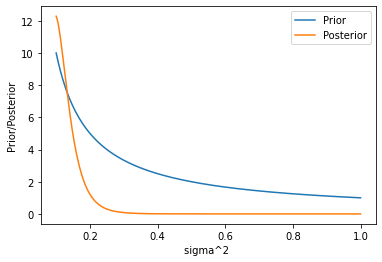
\includegraphics[width = 0.6\textwidth]{q6b.png}
  \caption{Posterior superimposed on the Normal prior}
\end{figure}
\noindent \emph{d.} To calculate a 90\% centered quantile based credible interval, we make use of the approach followed in Q.3., and we reuse the function defined and implemented in Q.3. Following a similar approach, we get lower and upper bounds of the quantiles as, $(q_{5}, q_{95}) = (0.10242307810098894, 0.21316013463489708)$. This converts to the following credible region on the posterior.
\begin{figure}[H]
  \centering
  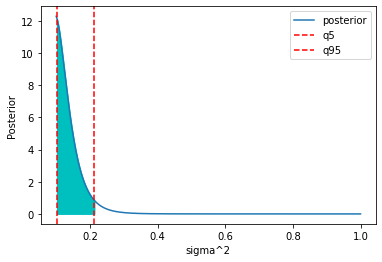
\includegraphics[width = 0.6\textwidth]{q6d.png}
  \caption{Quantile based credible regions on the posterior}
\end{figure}
\noindent \emph{e.} The HPD credible regions are defined in a similar fashion to the Quantile based credible regions. Let us consider a 100*(1 - $\alpha$) posterior credible region to be defined as,
\begin{equation}
  \nonumber
  \begin{aligned}
    C_{\theta, \alpha} & = \{\theta : Pr(C_{\theta}, \alpha \text{ }|\text{ } y_{1:n}) = 1 - \alpha, p(\theta_{1}\text{ }|\text{ }y_{1:n}) \geq p(\theta_{2}\text{ }|\text{ }y_{1:n}) \forall \theta_{1} \in C_{\theta}, \theta_{2} \in C_{\theta}^{c}\}\\
  \end{aligned}
\end{equation}
For calculating the HPD credible intervals, we make use of the implementation by PacktPublishing
on this link: \url{https://github.com/PacktPublishing/Bayesian-Analysis-with-Python/blob/master/Chapter%201/hpd%20(1).py}\\ \\
Using this, we calculate the HPD lower and upper bound values as $(\text{hpd}_{l}, \text{hpd}_{u}) = (0.1, 0.19)$. Now, using this interval, we plot the credible region as,
\begin{figure}[H]
  \centering
  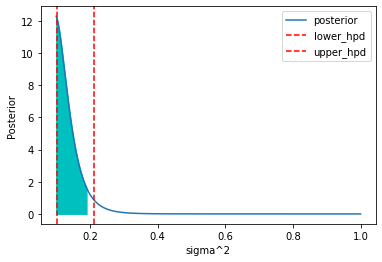
\includegraphics[width = 0.6\textwidth]{q6e.png}
  \caption{HPD based credible regions on the posterior}
\end{figure}
The code accomanying these graphs with detailed explanations and comments are attached with this assigment.
\end{document}
